\chapter{JSON Messaging with WebSocket}

\begin{figure}[h]
	\centering
    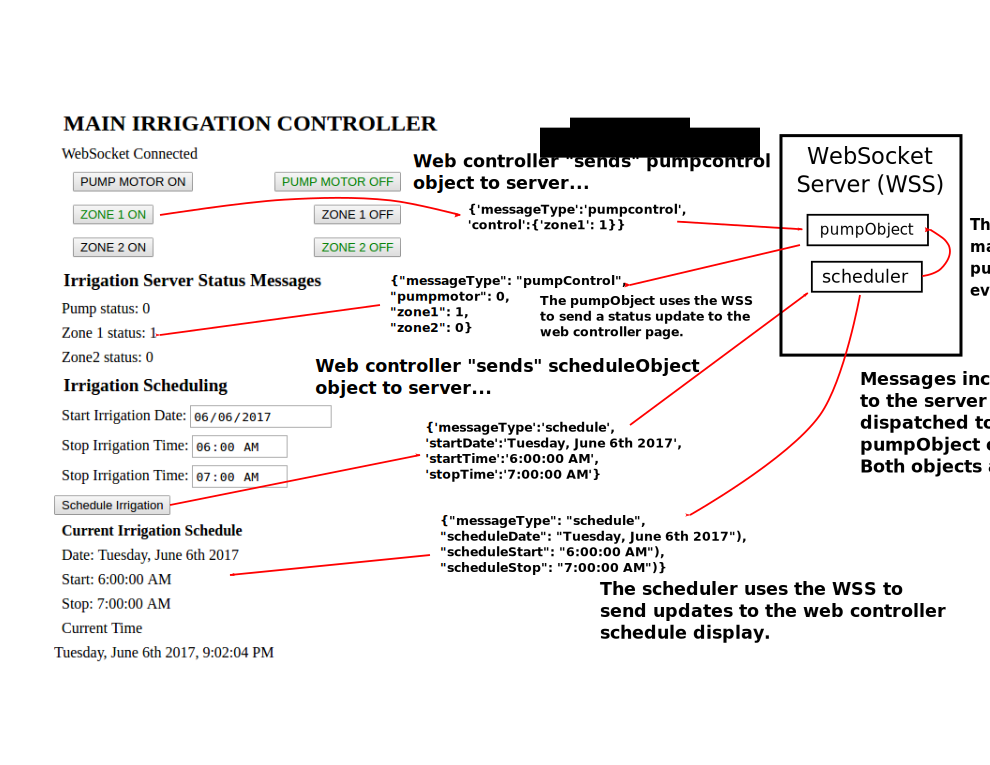
\includegraphics[width=1.0\textwidth]{diagrams/websocket_comms}
	\centering\bfseries
	\caption{JSON Objects are passed between the Web Page Controller and the 
	Server}
\end{figure}

The above diagram shows the flow of data between the web browser controller and 
the BBGW server.

``Javascript Object Notation'' (JSON) is used the format used for the 
messages.  These ``Objects'' are used as associative arrays would be 
used in other programming languages.  In fact, ES6 includes a formal 
associative array called Map.  However, JSON is a de-facto standard for this 
sort of simple message passing, and the JSON related tools are easy to use.

To send a JSON Object with WebSocket, it is first necessary to ``stringify'' 
the object.  This is done with the JSON.stringify() method.  On the receiving 
end, the JSON.parse() method is used to translate back to a Javascript Object.  
After that, the Object is used with the normal key/value syntax of Javascript.

\section{Example JSON Messages}

Thanks to WebSocket being bidirectional, it is easy to pass messages in both 
directions between the web browser controller and the server.  There are a 
total of four message types; two for browser to server and two for server to 
browser.

\subsection{Browser to Server Hardware Control Message}

This message indicates the device to be controlled and the desired state:

\begin{verbatim}
{'messageType':'pumpControl', 'control':{'zone1':1}}
\end{verbatim}

The key ``messageType'' indicates to the server that this message should be 
routed to the pumpActuator Object.  The ``control'' key's value is another JSON 
object, and this Object has as its key the device to be controlled, and the 
value is the desired state.

A little bit of ES6 Javascript trickery is involved to use this piece of 
incoming data:

\begin{verbatim}
Object.assign(pumpObject.pumpMapProxy, dataObject.control);
\end{verbatim}

The pumpActuator object has a data structure containing the current state of 
the zone solenoids and the pump motor.  The data structure is an ES6 ``Map'', 
which is a true associative array.

So what the Object.assign(arg1, arg2) method does is overwrite key:value pair 
located in arg1 with the key:value pair in arg2.

Due to the write being done through a Proxy Object, another function is called 
which physically changes the state of the correct GPIO, and the function then 
sends another object back to the web browser to update its status display.

The ES6 Proxy Object appears to be useful 
for managing state in Javascript based embedded devices.  The interested reader 
is encouraged to check out the documentation at this link:

\url{https://developer.mozilla.org/en-US/docs/Web/JavaScript/Reference/Global_Objects/Proxy}

\subsection{Server to Browser Hardware Status Message}

When the project was first started, the buttons in the web browser to turn the 
hardware components on and off was simple DOM updates of the button colors.

However, this does not indicate the true state of the hardware in the case of a 
communications breakdown between browser and server.

The design was revised to update button indicators only upon receipt of a 
message from the server indicating a successful hardware state change.

The pumpActuator object emits ``pumpStatusMessage'', and then only if a 
WebSocket is open the status message is sent to the browser.  The web browser 
parses the message and uses DOM Javascript manipulation to update the displayed 
hardware status.

\begin{verbatim}
{'messageType':'pumpControl', 'pumpmotor':0, 'zone1':1, 'zone2':0}
\end{verbatim}

\subsection{Browser to Server Scheduling Message}

The system user can input a date, start, and stop times for irrigation to 
happen automatically in the future.  Simple HTML5 form fields are used to 
gather the user's input, and then a ``Schedule Irrigation'' button is clicked.  
If a valid WebSocket is open, a scheduling JSON object is sent to the server.

\begin{verbatim}
{'messageType':'schedule', 'scheduleData':'Tuesday June 6th 2017',
'scheduleStart':'6:00:00 AM', 'scheduleStop':'7:00:00'}
\end{verbatim}

The websocketserver determines the ``messageType'' is schedule, and then 
dispatches the message to the Scheduler Object.  

\subsection{Server to Browser Schedule Display Update Message}

The Scheduler has the necessary logic to drive the hardware per the schedule.

The browser's displayed schedule is updated by the server, not by the browser.  
Thus the server sends the scheduling message back to the browser, but only if 
the message is first processed by the Scheduler object and also a valid 
WebSocket is open.  The message is identical to the browser to server message.

The scheduling display is updated using DOM Javascript methods.